%%%%%%%%%%%%%%%%%%%%%%%%%%%%%%%%%%%%%%%%%%%%%%%%%
%%%%   SECTION 3b — Results and Discussion   %%%%
%%%%%%%%%%%%%%%%%%%%%%%%%%%%%%%%%%%%%%%%%%%%%%%%%

\subsection{Results and Discussion}
\label{sec:eval_results}

% ── 3b.1  QUERY FIELD ABLATION ────────────────────────────────────────────────
\subsubsection{Query Field Ablation (BM25, Train Set)}

The first step selects the query formulation.  Six combinations of the topic
fields were tested on 32 train queries using BM25 with default parameters as
the proxy retriever.  Table~\ref{tab:ablation} and
Figure~\ref{fig:field_ablation} show the results.

\textbf{Winner: \texttt{topic+question}} — NDCG@100=0.7833, MAP=0.5843.
The \texttt{narrative} field adds noise (instructions and qualifiers not found
in abstracts); \texttt{topic} alone misses clinical context synonyms.
The \texttt{topic+question} concatenation is locked for all subsequent
experiments.

\begin{table}[htbp]
\centering
\caption{Query field ablation — BM25 default on 32 train topics.
         Bold = winner; NDCG@100 is the selection criterion.}
\label{tab:ablation}
\begin{tabular}{lcccc}
  \hline
  \textbf{Field} & \textbf{NDCG@100} & \textbf{MAP} & \textbf{MRR}
                 & \textbf{P@10} \\
  \hline
  topic only       & 0.7381 & 0.5334 & \textbf{0.8255} & 0.6313 \\
  question only    & 0.7174 & 0.4988 & 0.8135 & 0.6562 \\
  narrative only   & 0.6099 & 0.3900 & 0.6890 & 0.5500 \\
  \textbf{topic+question}   & \textbf{0.7833} & \textbf{0.5843} & 0.8229 & \textbf{0.7000} \\
  topic+narrative  & 0.7205 & 0.5145 & 0.7083 & 0.6500 \\
  all three        & 0.7611 & 0.5673 & 0.7240 & 0.7031 \\
  \hline
\end{tabular}
\end{table}

\begin{figure}[htbp]
  \centering
  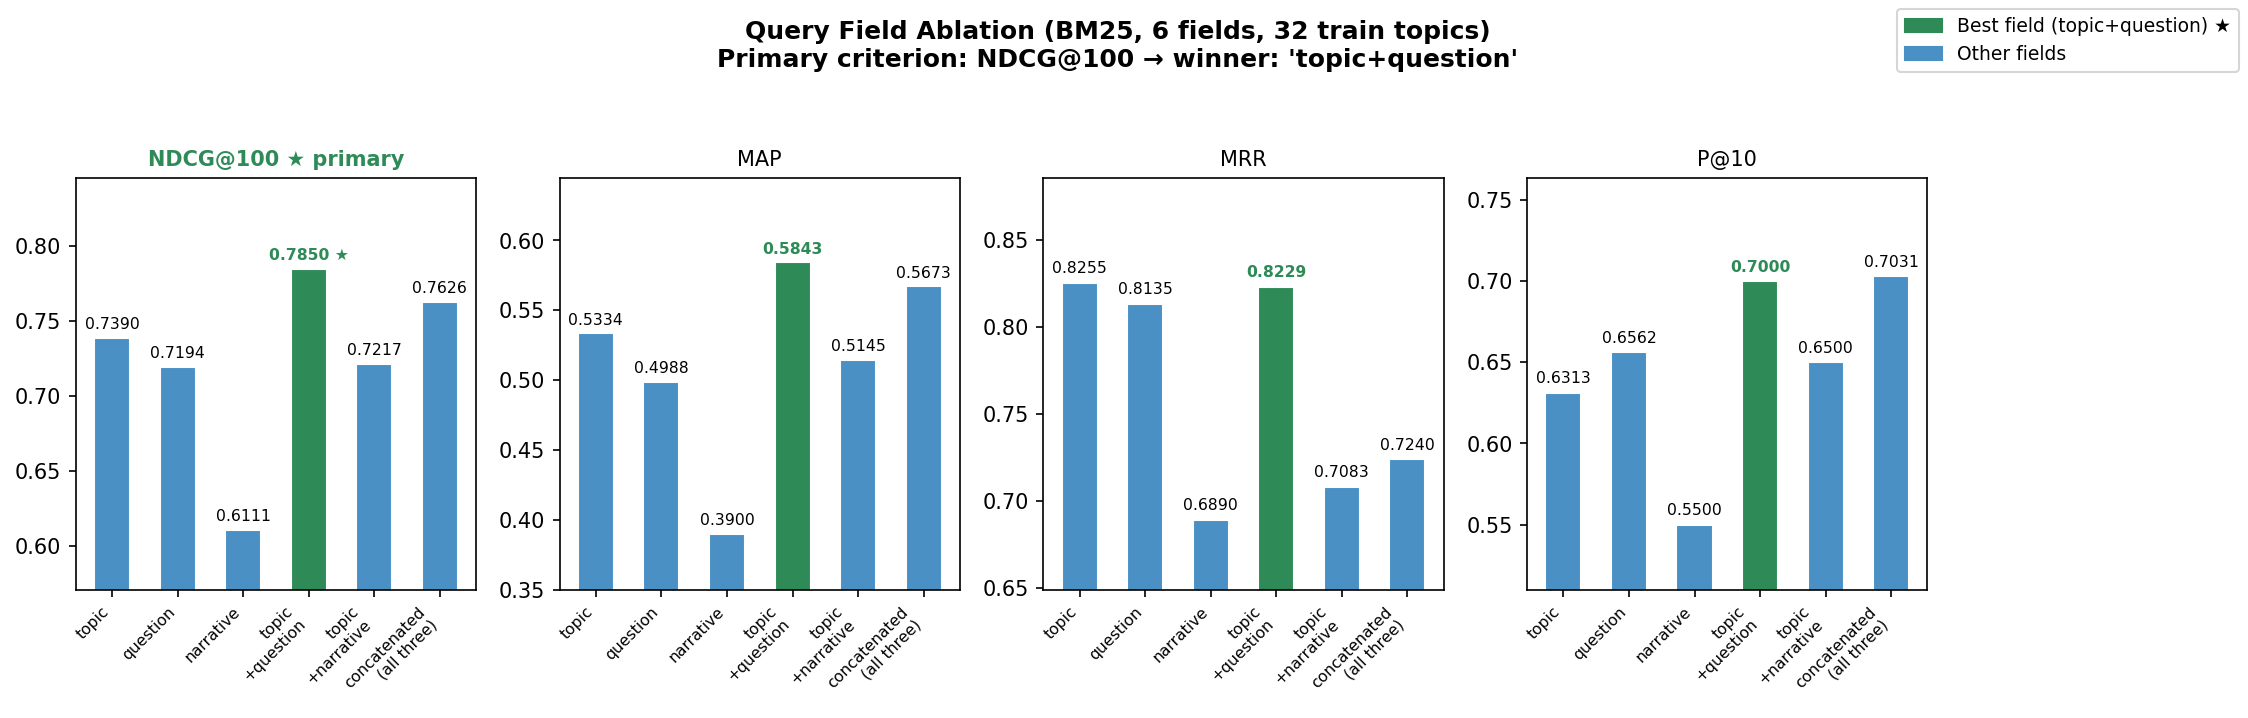
\includegraphics[width=\linewidth]{images/field_ablation.png}
  \caption{Field ablation results — NDCG@100 (primary) and MAP for each
           query formulation on the 32 train topics. \texttt{topic+question}
           achieves the highest NDCG@100 and is locked for all subsequent
           experiments.}
  \label{fig:field_ablation}
\end{figure}

% ── 3b.2  HYPERPARAMETER TUNING ───────────────────────────────────────────────
\subsubsection{Hyperparameter Tuning (5-Fold CV, Train Set)}

All sweeps use the locked \texttt{topic+question} field from
§\ref{sec:eval_setup}.

\paragraph{BM25:} $k_1 \times b$ grid, 24 configurations:
winner $k_1$=1.5, $b$=1.0 — NDCG@100=\textbf{0.7989}
($\Delta$=+0.0088 vs default $k_1$=1.2, $b$=0.75 at 0.7901).
High $b$=1.0 means full length normalisation: longer, more comprehensive
abstracts are rewarded rather than penalised.
See Figure~\ref{fig:bm25_sweep}.

\begin{figure}[htbp]
  \centering
  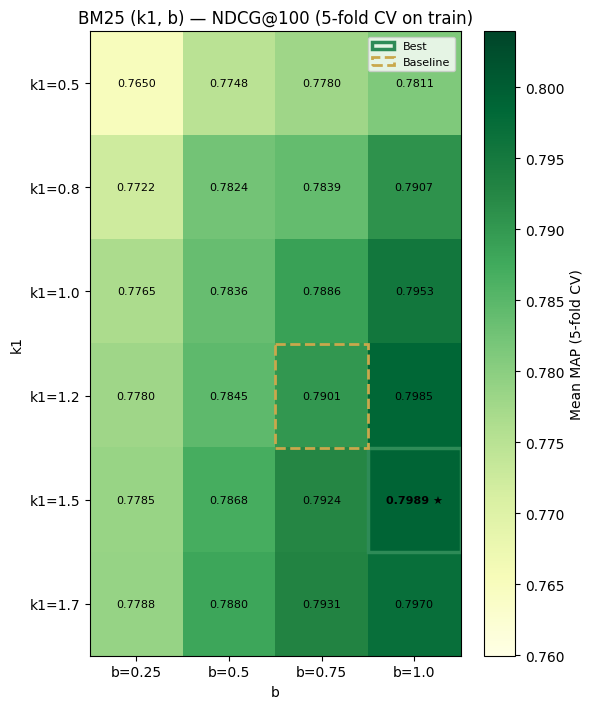
\includegraphics[width=0.70\linewidth]{images/bm25_param_sweep.png}
  \caption{BM25 $k_1$/$b$ sweep — mean CV NDCG@100. Winner: $k_1$=1.5,
           $b$=1.0.}
  \label{fig:bm25_sweep}
\end{figure}

\paragraph{LM Dirichlet:}
$\mu \in \{50, 75, 100, 125, 200, 500, 1000, 2000\}$:
CV winner $\mu = 100$ — NDCG@100 = 0.7706
($\Delta = {+}0.0196$ vs default $\mu = 2000$ at 0.7510).
The default $\mu$=2{,}000 is $\approx$13$\times$ the mean document length
(150~words) and over-smooths every abstract.
See Figure~\ref{fig:lmdir_sweep}.

\begin{figure}[htbp]
  \centering
  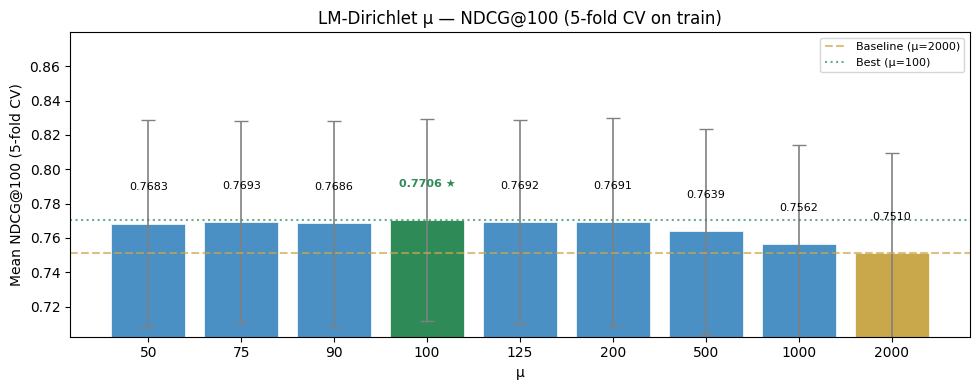
\includegraphics[width=0.92\linewidth]{images/lmdir_mu_sweep.png}
  \caption{LM-Dir $\mu$ sweep — mean CV NDCG@100. Default $\mu$=2000
           drastically under-performs; winner is $\mu$=100.}
  \label{fig:lmdir_sweep}
\end{figure}

\paragraph{LM Jelinek-Mercer:}
Seven values of $\lambda$ between 0.1 and 0.9 were tested (extended grid);
winner $\lambda = 0.65$ — NDCG@100 = 0.7754
($\lambda = 0.7$ at 0.7746; the extended grid confirms 0.65 edges ahead
by $\Delta = {+}0.0008$, within noise).
See Figure~\ref{fig:lmjm_sweep}.

\begin{figure}[htbp]
  \centering
  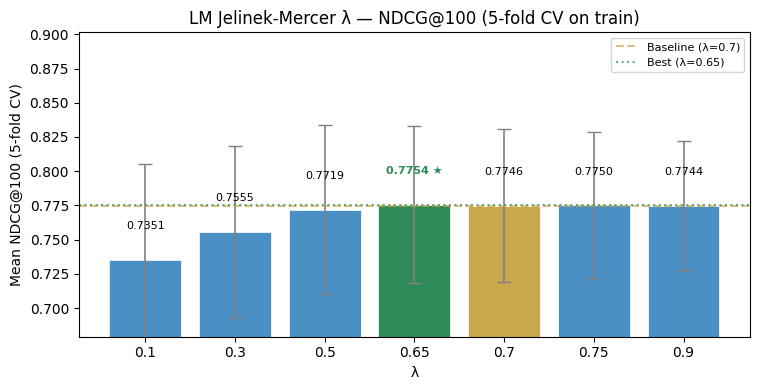
\includegraphics[width=0.82\linewidth]{images/lmjm_lambda_sweep.png}
  \caption{LM-JM $\lambda$ sweep — NDCG@100 plateaus in the 0.65--0.75 range;
           extended grid winner $\lambda$=0.65.}
  \label{fig:lmjm_sweep}
\end{figure}

\paragraph{Dense encoder comparison:}
MedCPT wins over multi-qa-mpnet, SPECTER-2, and
msmarco-distilbert — NDCG@100=\textbf{0.8273}
($\Delta$=+0.0825 vs msmarco baseline at 0.7448).
Trained on 23M PubMed click-through pairs, MedCPT is an exact domain match
for our task.  Encoder selection used brute-force exact cosine in Python
(not HNSW) to eliminate index-approximation noise; each encoder's best
pooling mode (CLS for MedCPT/SPECTER-2, mean-no-special for msmarco/multi-qa)
was determined first (see §\ref{sec:phase1}).
Full results are in Table~\ref{tab:encoder_comp} and
Figure~\ref{fig:encoder_sweep}.

\begin{table}[htbp]
\centering
\caption{Dense encoder comparison — 5-fold CV on 32 train topics (each
         encoder uses its best pooling mode from Table~\ref{tab:pooling}).
         Bold = best per column; $\star$ = selected encoder.
         MedCPT wins the primary metric (NDCG@100) despite multi-qa
         leading on MAP and P@10.}
\label{tab:encoder_comp}
\begin{tabular}{lcccc}
  \hline
  \textbf{Encoder} & \textbf{NDCG@100} & \textbf{MAP} & \textbf{MRR}
                   & \textbf{P@10} \\
  \hline
  MedCPT $\star$         & \textbf{0.8273} & 0.6209          & 0.8802          & 0.7094 \\
  multi-qa               & 0.8236          & \textbf{0.6435} & 0.8698          & \textbf{0.7719} \\
  msmarco (baseline)     & 0.7448          & 0.5403          & 0.8568          & 0.7469 \\
  SPECTER-2              & 0.7292          & 0.5177          & \textbf{0.8854} & 0.7500 \\
  \hline
\end{tabular}
\end{table}

\begin{figure}[htbp]
  \centering
  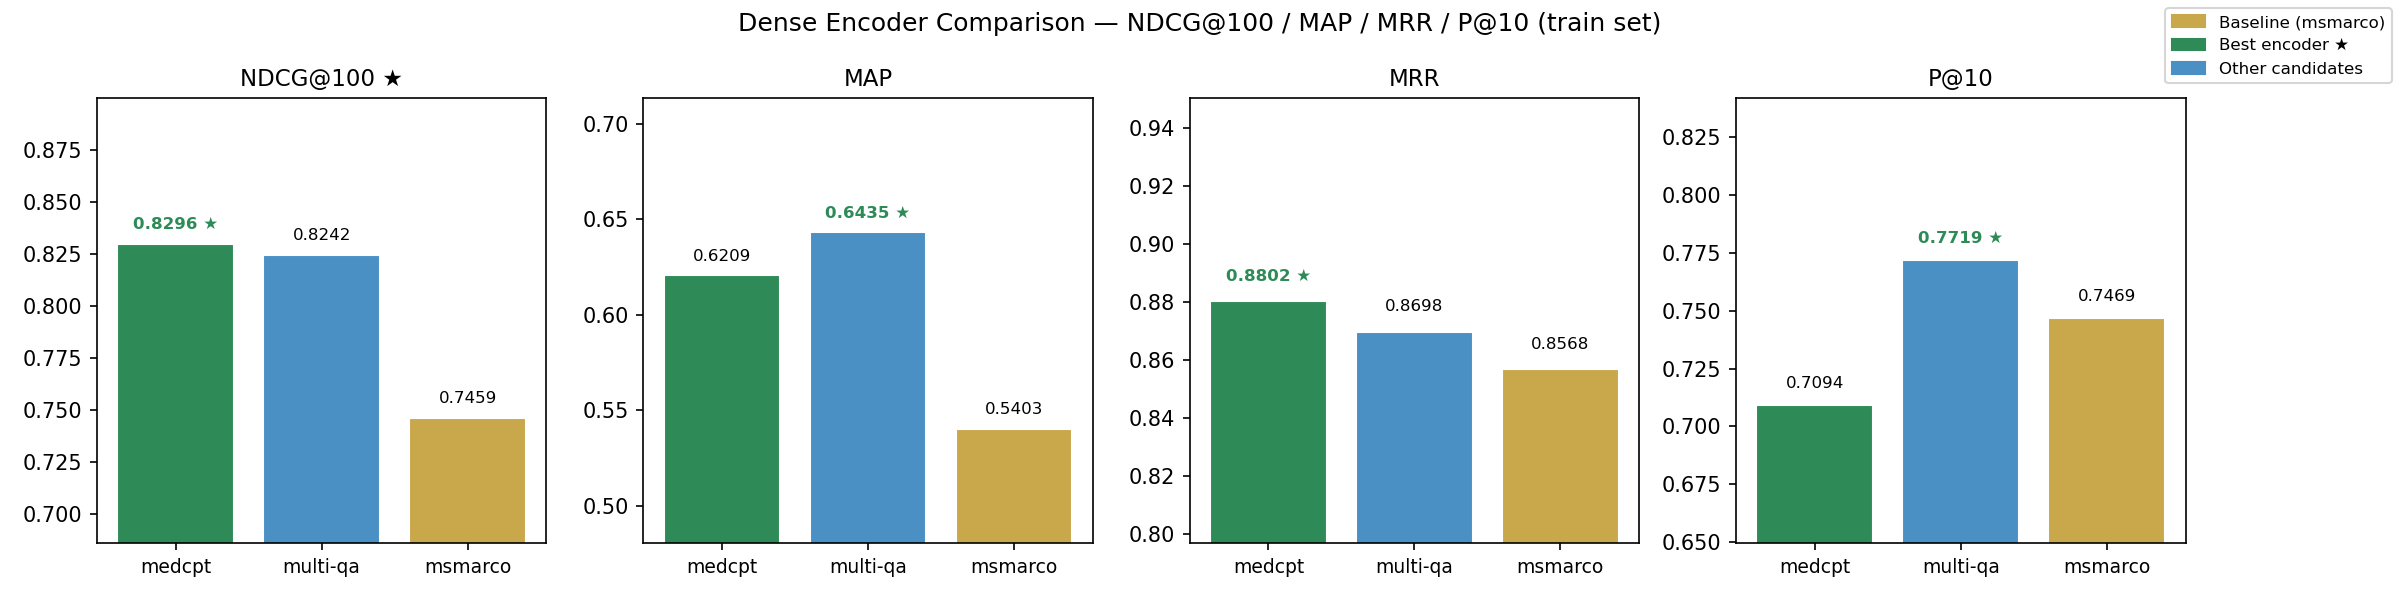
\includegraphics[width=\linewidth]{images/encoder_comparison.png}
  \caption{Encoder comparison — NDCG@100 on 32 train topics. MedCPT
           dominates (+0.0825 over msmarco baseline).}
  \label{fig:encoder_sweep}
\end{figure}

\paragraph{RRF pair sweep:}
Nine strategy pairs were tested across three $k$ values (30, 60, 90) in
5-fold CV.  The best lexical pair was BM25+LM-Dir at $k$=90
(NDCG@100=0.7907); however, no RRF pair surpasses KNN(MedCPT) solo
(0.8273) on the train CV leaderboard.
See Figure~\ref{fig:rrf_sweep}.

\begin{figure}[htbp]
  \centering
  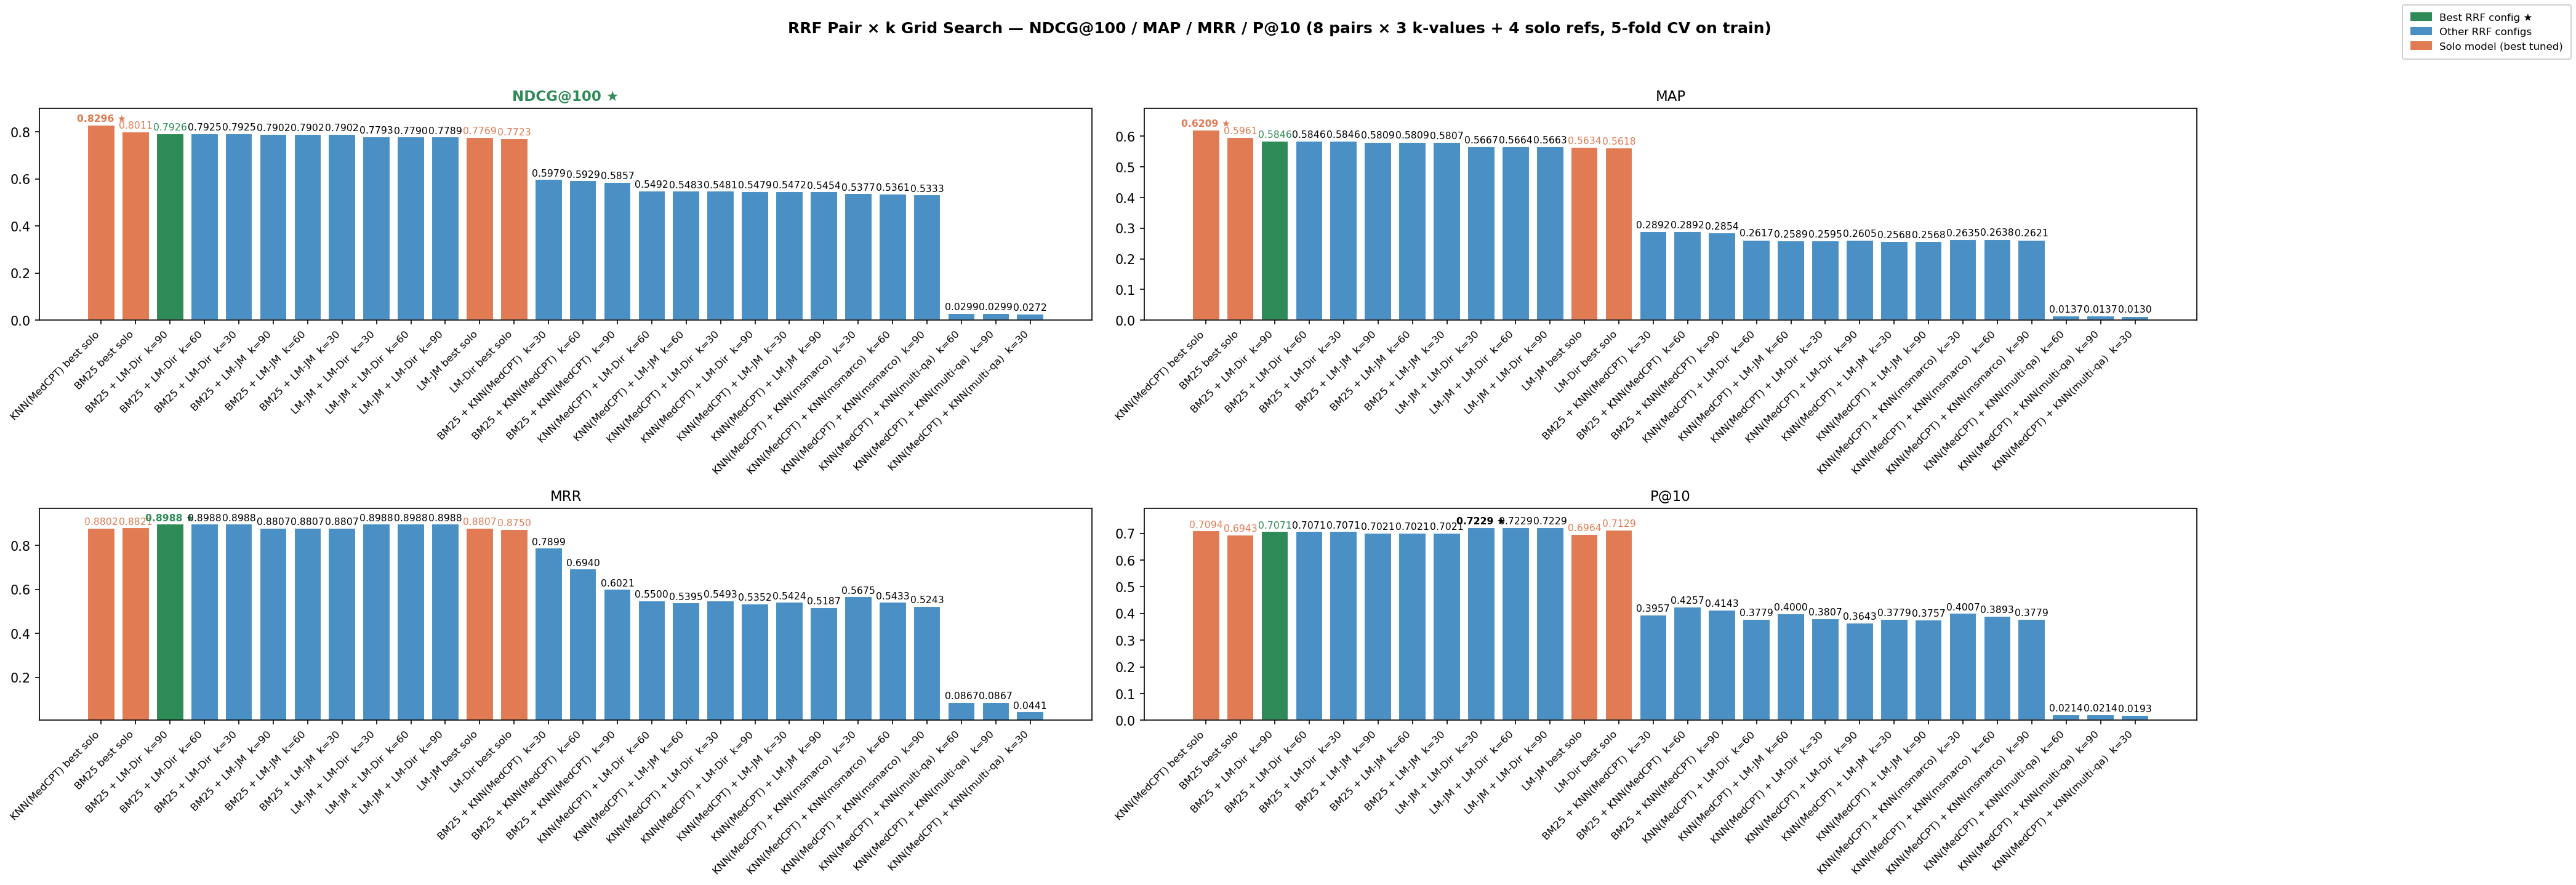
\includegraphics[width=\linewidth]{images/rrf_pair_sweep.png}
  \caption{RRF pair sweep — 9 strategy pairs $\times$ 3 $k$ values, 5-fold CV.
           Lexical pairs (BM25+LM-Dir, $k$=90, NDCG@100=0.7907) outperform
           KNN fusions at the rank-level.}
  \label{fig:rrf_sweep}
\end{figure}

\paragraph{Train CV summary:}
Table~\ref{tab:leaderboard} ranks all tuned strategies by NDCG@100
on the train CV; KNN(MedCPT) is the overall winner.
Figure~\ref{fig:tuning_summary} visualises the baseline-to-tuned gain for
each model; encoder selection (MedCPT) yields the largest gain,
followed by LM-Dir correction ($\mu = 100$).

\begin{table}[htbp]
\centering
\caption{Train CV leaderboard — all tuned solo strategies and the best RRF
         pair, ranked by NDCG@100 (5-fold CV on 32 train topics).
         KNN(MedCPT) is the overall winner; no RRF pair surpasses it.}
\label{tab:leaderboard}
\begin{tabular}{clcc}
  \hline
  \textbf{Rank} & \textbf{Strategy} & \textbf{NDCG@100} & \textbf{MAP} \\
  \hline
  1 & KNN (MedCPT)               & \textbf{0.8273} & \textbf{0.6209} \\
  2 & BM25 ($k_1$=1.5, $b$=1.0)  & 0.7989          & 0.5961 \\
  3 & RRF (BM25+LM-Dir, $k$=90)  & 0.7907          & 0.5846 \\
  4 & LM-JM ($\lambda$=0.65)     & 0.7754          & 0.5636 \\
  5 & LM-Dir ($\mu$=100)         & 0.7706          & 0.5618 \\
  \hline
\end{tabular}
\end{table}

\begin{figure}[htbp]
  \centering
  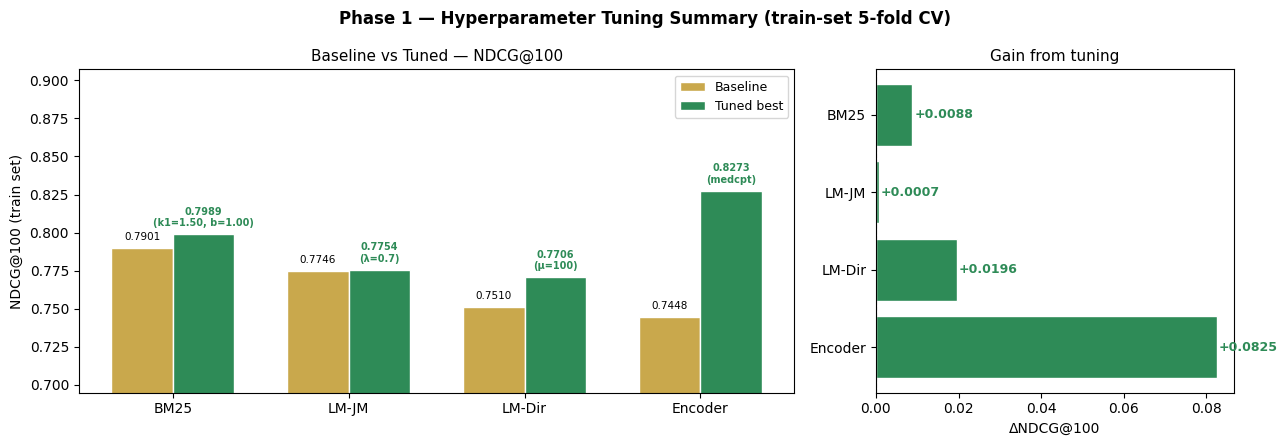
\includegraphics[width=\linewidth]{images/tuning_summary.png}
  \caption{Tuning summary: baseline vs.\ tuned NDCG@100 for every model
           (5-fold CV on 32 train topics). Encoder selection (MedCPT) yields
           the largest gain ($\Delta$NDCG@100=+0.0825 over msmarco); LM-Dir
           correction ($\mu$=100) yields the second-largest (+0.0196).}
  \label{fig:tuning_summary}
\end{figure}

% ── 3b.3  LOCKED CONFIGURATION ────────────────────────────────────────────────
\subsubsection{Locked Configuration}

All hyperparameters are locked after the train-set sweeps described above.
Table~\ref{tab:locked_config} lists the final configuration passed to
Phase~2.

\begin{table}[htbp]
\centering
\caption{Locked Phase~1 configuration.  All values selected on the 32-query
         train set (5-fold CV); test set touched once.}
\label{tab:locked_config}
\begin{tabular}{ll}
  \hline
  \textbf{Parameter} & \textbf{Value} \\
  \hline
  Query field               & \texttt{topic+question} \\
  BM25 $k_1$, $b$           & 1.5, 1.0 \quad (CV NDCG@100=0.7989) \\
  LM-JM $\lambda$           & 0.65 \quad (CV NDCG@100=0.7754) \\
  LM-Dir $\mu$              & 100 \quad (CV NDCG@100=0.7706) \\
  Dense encoder             & MedCPT (asymmetric, CLS pooling) \\
  RRF pair                  & BM25 + KNN(MedCPT), $k$=60 \\
  Best overall (train CV)   & KNN(MedCPT) — NDCG@100=0.8273 \\
  Best overall (test)       & RRF (BM25+MedCPT) — NDCG@100=0.8245 \\
  \hline
\end{tabular}
\end{table}

% ── 3b.4  TEST SET RESULTS ────────────────────────────────────────────────────
\subsubsection{Test Set Results (33 Topics)}

All strategies are evaluated once on the held-out test set after all
parameters are locked.  All use \texttt{topic+question}; top-100 results
per query.  Table~\ref{tab:test_results} compares baseline (default
parameters) against tuned configurations across all five metrics.
Figure~\ref{fig:tuning_gain} shows the per-strategy tuning gain.

\begin{table}[htbp]
\centering
\caption{Baseline (default parameters) vs tuned — all 5 metrics on the
         33-query test set. NDCG@100 is the primary metric (graded qrels).
         Bold = best per column.}
\label{tab:test_results}
\begin{tabular}{lccccc}
  \hline
  \textbf{Strategy} & \textbf{NDCG@100} & \textbf{MAP} & \textbf{MRR}
                    & \textbf{P@10} & \textbf{R@100} \\
  \hline
  \multicolumn{6}{l}{\textit{Baseline (default parameters)}} \\
  BM25 ($k_1$=1.2, $b$=0.75)   & 0.7756 & 0.5695 & 0.7712 & 0.6333 & 0.8594 \\
  LM-JM ($\lambda$=0.7)         & 0.7586 & 0.5431 & 0.7848 & 0.6333 & 0.8303 \\
  LM-Dir ($\mu$=2000)           & 0.7341 & 0.5149 & 0.7740 & 0.6212 & 0.8100 \\
  KNN (msmarco)                 & 0.7576 & 0.5561 & 0.8384 & \textbf{0.6879} & 0.8933 \\
  RRF (default)                 & 0.8114 & 0.6100 & 0.8141 & 0.6667 & 0.8921 \\
  \hline
  \multicolumn{6}{l}{\textit{Tuned (locked parameters)}} \\
  BM25 ($k_1$=1.5, $b$=1.0)    & 0.7742 & 0.5677 & 0.7141 & 0.6333 & 0.8600 \\
  LM-JM ($\lambda$=0.65)        & 0.7569 & 0.5413 & 0.7864 & 0.6212 & 0.8303 \\
  LM-Dir ($\mu$=100)            & 0.7555 & 0.5428 & 0.7773 & 0.6061 & 0.8270 \\
  \textbf{KNN (MedCPT)}         & 0.8077 & 0.6143 & 0.8000 & 0.6788 & \textbf{0.8933} \\
  \textbf{RRF (BM25+MedCPT)}   & \textbf{0.8245} & \textbf{0.6266}
                                & \textbf{0.8394} & 0.6515 & \textbf{0.9142} \\
  \hline
\end{tabular}
\smallskip\par\noindent\small
KNN(MedCPT) is the \emph{train CV winner} (NDCG@100=0.8273).
RRF (BM25+MedCPT, $k$=60) achieves the highest \emph{test-set} NDCG@100=0.8245.
\end{table}

\begin{figure}[htbp]
  \centering
  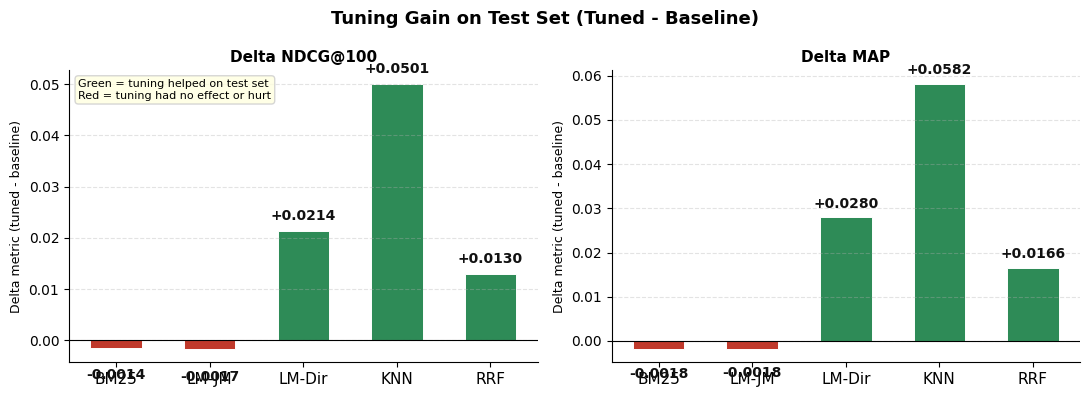
\includegraphics[width=\linewidth]{images/tuning_gain_test.png}
  \caption{Tuning gain on the test set ($\Delta$NDCG@100 and $\Delta$MAP,
           tuned $-$ baseline). KNN and RRF gain significantly; BM25 tuning
           yields no measurable gain ($\Delta$NDCG@100\,=\,$-$0.0014).}
  \label{fig:tuning_gain}
\end{figure}

\paragraph{Key observations:}
KNN\,(MedCPT) wins on the train CV
(NDCG@100 = 0.8273) and achieves
NDCG@100 = 0.8077, MAP = 0.6143, R@100 = 0.8933
on the test set, making it the locked Phase~2 backbone.
RRF (BM25 + MedCPT, $k = 60$) pushes the test NDCG@100 further to
0.8245 by fusing complementary lexical and dense signals.
Selecting MedCPT is the single most impactful change overall:
$\Delta$NDCG@100 = +0.0501 versus the msmarco KNN baseline on test
($0.7576 \to 0.8077$).
By contrast, BM25 tuning has minimal effect
($\Delta = -0.0014$ on test — tuning slightly hurt generalisation),
while LM-Dir tuning delivers a clear improvement
($\mu = 100$ versus $\mu = 2{,}000$: $0.7341 \to 0.7555$, +0.0214).
The R@100 of 0.8933 for KNN\,(MedCPT) covers more than 89\% of relevant
documents, providing a strong evidence pool for Phase~2 generation.

% ── 3b.5  PER-TOPIC ANALYSIS ─────────────────────────────────────────────────
\subsubsection{Per-Topic Analysis}

AP ranges widely across topics, revealing high sensitivity to query phrasing
and topic specificity.  Figure~\ref{fig:individual_pr} shows per-topic
PR curves for KNN\,(MedCPT), the locked Phase~2 strategy.
The best-performing topic is~170 (isoniazid hepatotoxicity,
AP\,=\,0.8961), whose specific clinical and drug terminology aligns well
with PubMed vocabulary.
The median case is topic~120 (causes of facial numbness, AP\,=\,0.6277),
while the hardest is topic~140 (spontaneous hand fractures, AP\,=\,0.1168),
where the broad, ambiguous query leaves few relevant PMIDs recoverable in
the top~100.
An informal IDF analysis suggests that low-IDF terms such as ``treatment''
and ``patient'' correlate with low AP, whereas disease-specific or
drug/gene-symbol terms tend to produce higher scores.

\begin{figure}[htbp]
  \centering
  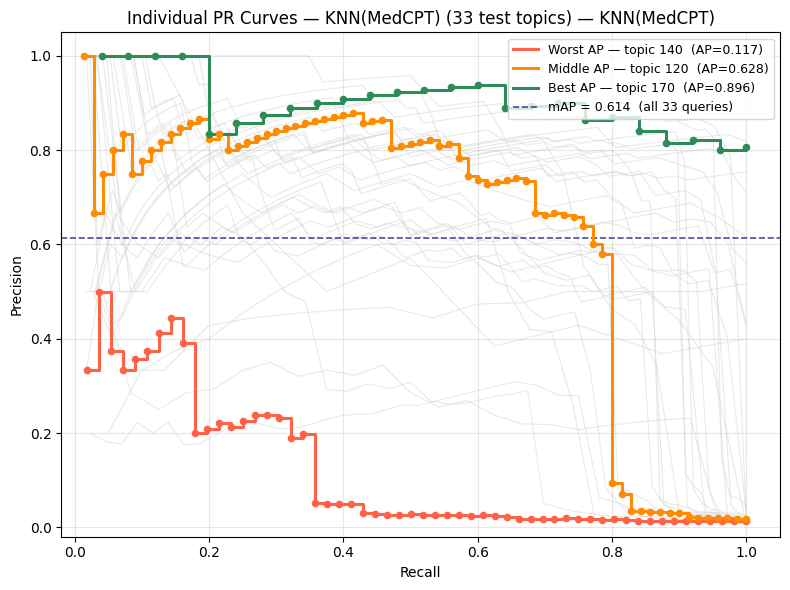
\includegraphics[width=0.85\linewidth]{images/individual_pr_curves.png}
  \caption{Per-topic PR curves for KNN(MedCPT) on all 33 test topics.
           Green = best topic (170 — isoniazid hepatotoxicity, AP=0.8961);
           red = worst topic (140 — spontaneous hand fractures, AP=0.1168);
           orange = median topic (120 — causes of facial numbness, AP=0.6277).
           Gray curves = remaining 30 topics.
           Dashed navy = mean AP (MAP=0.6143).
           Wide spread indicates high sensitivity to topic vocabulary.}
  \label{fig:individual_pr}
\end{figure}

Figure~\ref{fig:ap_boxplot} shows the AP distribution across all strategies.
RRF (tuned) achieves the highest median AP and the least variance, confirming
its robustness.  Note that the median AP for KNN(MedCPT) is slightly lower
than for RRF(tuned) because RRF fuses complementary lexical and dense
signals: BM25 rescues topics where the dense encoder struggles with
out-of-vocabulary biomedical terms, raising the floor AP.

\begin{figure}[htbp]
  \centering
  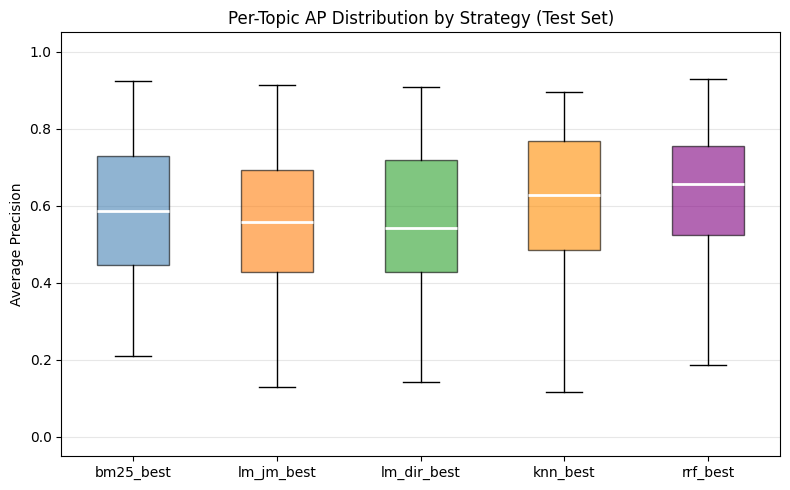
\includegraphics[width=0.80\linewidth]{images/ap_boxplot.png}
  \caption{Per-topic AP distribution across all strategies (test set, 33
           topics). RRF (tuned) achieves the highest median AP and the least
           variance. Wide IQR reflects inherent topic-difficulty spread.
           Outliers below the whisker correspond to hard topics (AP$<$0.3).}
  \label{fig:ap_boxplot}
\end{figure}

% ── 3b.6  PRECISION-RECALL ANALYSIS ──────────────────────────────────────────
\subsubsection{Precision-Recall Analysis (MAP)}

PR curves are computed as 11-point interpolated means across all 33 test
topics (Lab03 protocol).  The area under each curve approximates MAP —
a larger area indicates better overall ranking quality.

Figure~\ref{fig:pr_curves} shows the mean interpolated PR curves for all
strategies.  RRF (tuned) and KNN(MedCPT) dominate across the full recall
range.  The lexical LM variants show steeper early-recall drops, reflecting
their weaker semantic matching.  At high recall levels ($>$0.6), RRF
maintains notably higher precision than any single model, again illustrating
the benefit of fusing complementary retrieval signals.

\begin{figure}[htbp]
  \centering
  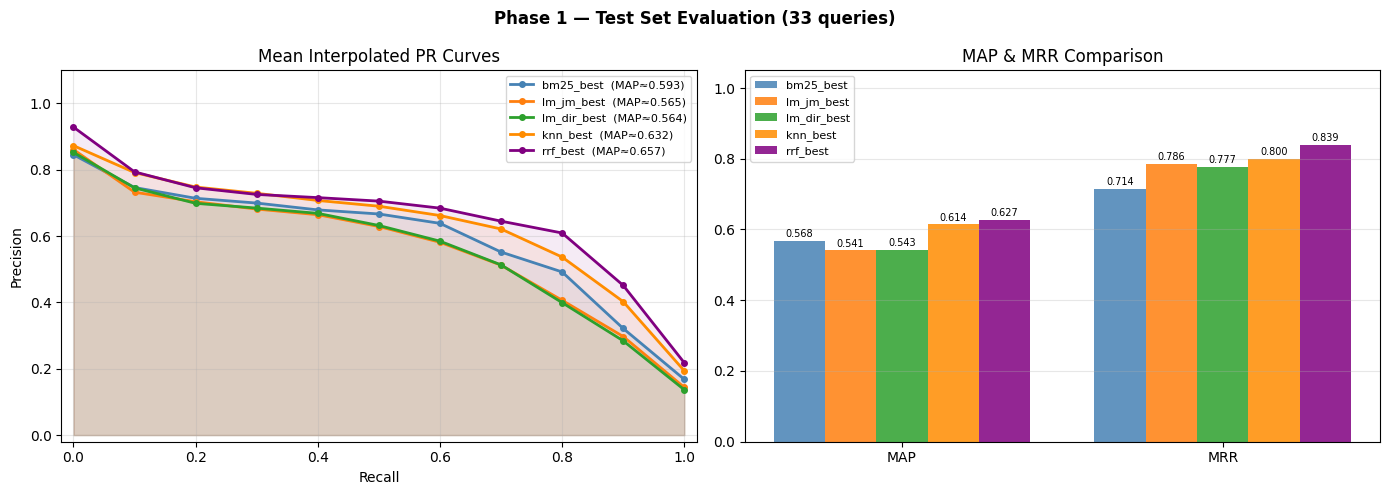
\includegraphics[width=\linewidth]{images/pr_curves.png}
  \caption{Mean interpolated PR curves for all strategies on the 33-query
           test set (left) with MAP/MRR bar chart (right). RRF (tuned) and
           KNN (MedCPT) dominate across the full recall range. LM variants
           show steeper early-recall drops.}
  \label{fig:pr_curves}
\end{figure}
